\section{Appendix: Gradient Estimator Derivations \& Correctness Proofs}
\label{sec:appendix_proofs}

\newtheorem{lemma}{Lemma}
\newtheorem{theorem}{Theorem}

\subsection{Derivation of Unified Gradient Estimator (Equation~\ref{eq:hybridEstimator})}
\label{sec:appendix:estDerivation}

\begin{align}
\gradparams \elbo
%
&= \gradparams \expect_\reparamDist [ \log p(\xformedVars, \observedVars) - \log \guide(\xformedVars | \observedVars) ]\nonumber\\
%
&= \gradparams \int_\reparamVars \reparamDist(\reparamVars | \observedVars) ( \log p(\xformedVars, \observedVars) - \log \guide(\xformedVars | \observedVars) )\nonumber\\
%
&= \int_\reparamVars \gradparams \reparamDist(\reparamVars | \observedVars) ( \log p(\xformedVars, \observedVars) - \log \guide(\xformedVars | \observedVars) ) + \reparamDist(\reparamVars | \observedVars) \gradparams ( \log p(\xformedVars, \observedVars) - \log \guide(\xformedVars | \observedVars) )\nonumber \\
%
\label{eq:estDerivation_trick}
&= \int_\reparamVars \reparamDist(\reparamVars | \observedVars) \gradparams \log \reparamDist(\reparamVars | \observedVars) ( \log p(\xformedVars, \observedVars) - \log \guide(\xformedVars | \observedVars) ) + \reparamDist(\reparamVars | \observedVars) \gradparams ( \log p(\xformedVars, \observedVars) - \log \guide(\xformedVars | \observedVars) ) \\
%
&= \expect_\reparamDist [ \gradparams \log \reparamDist(\reparamVars | \observedVars) ( \log p(\xformedVars, \observedVars) - \log \guide(\xformedVars | \observedVars) ) + \gradparams( \log p(\xformedVars, \observedVars) - \log \guide(\xformedVars | \observedVars) )]\nonumber\\
%
&= \expect_\reparamDist [ \gradparams \log \reparamDist(\reparamVars | \observedVars) W(\reparamVars, \observedVars) + \gradparams \log p(\xformedVars, \observedVars) - \gradparams \log \guide(\xformedVars | \observedVars) ]\nonumber
\end{align}
Line~\ref{eq:estDerivation_trick} makes use of the identity $\nabla f(x) = f(x) \nabla \log f(x)$.
\ndg{need to define $W$}

\subsection{Zero Expectation Identities}
\label{sec:appendix:zeroexp}

In what follows, we will make frequent use of the following:

\begin{lemma}
If $f(x)$ is a probability distribution, then:

\begin{equation*}
\expect_f[\nabla \log f(x)] = 0
\end{equation*}
\label{lem:zeroexp}
\end{lemma}
%%%
\begin{proof}
\begin{equation*}
\expect_f[\nabla \log f(x)]
%
= \int_x f(x) \nabla \log f(x)
%
= \int_x \nabla f(x)
%
= \nabla \int_x f(x)
%
= \nabla 1
%
= 0
\end{equation*}
\end{proof}

\begin{lemma}
For a discrete random choice $\reparamVar_i$ and a function $f(\reparamVars_{<i}, \observedVars)$:
%
\begin{equation*}
\expect_\reparamDist [ \gradparams \log \guide(\reparamXform_i(\reparamVar_i) | \reparamXform(\reparamVars_{<i}), \observedVars) f(\reparamVars_{<i}, \observedVars) ] = 0
\end{equation*}
\label{lem:zeroexp2}
\end{lemma}
%%%
\begin{proof}
\begin{align*}
\expect_\reparamDist [ \gradparams \log \guide(\reparamXform_i(\reparamVar_i) | \reparamXform(\reparamVars_{<i}), \observedVars) f(\reparamVars_{<i}, \observedVars) ]
%
&= \int_\reparamVars \reparamDist(\reparamVars | \observedVars) \gradparams \log \guide(\reparamXform_i(\reparamVar_i) | \reparamXform(\reparamVars_{<i}), \observedVars) f(\reparamVars_{<i}, \observedVars)\\
%
&= \int_\reparamVars \reparamDist(\reparamVars | \observedVars) \gradparams \log \reparamDist(\reparamVar_i | \reparamVars_{<i}, \observedVars) f(\reparamVars_{<i}, \observedVars)\\
%
&= \int_{\reparamVars_{<i}} \reparamDist(\reparamVars_{<i} | \observedVars) f(\reparamVars_{<i}, \observedVars) \sum_{\reparamVar_i} \reparamDist(\reparamVar_i | \reparamVars_{<i}, \observedVars) \gradparams \log \reparamDist(\reparamVar_i | \reparamVars_{<i}, \observedVars) \int_{\reparamVars_{>i}} \reparamDist(\reparamVars_{>i} | \reparamVars_{\leq i}, \observedVars)\\
%
&= \int_{\reparamVars_{<i}} \reparamDist(\reparamVars_{<i} | \observedVars) f(\reparamVars_{<i}, \observedVars) \cdot \expect_{\reparamDist} [ \gradparams \log \reparamDist(\reparamVar_i | \reparamVars_{<i}, \observedVars) ] \cdot 1\\
%
&= \int_{\reparamVars_{<i}} \reparamDist(\reparamVars_{<i} | \observedVars) f(\reparamVars_{<i}, \observedVars) \cdot 0 = 0
\end{align*}
where the last line makes use of Lemma~\ref{lem:zeroexp}.
\end{proof}

\subsection{Variance Reduction Step 1: Zero Expectation $W$ Terms}

In this section, we show that for each random choice $i$, we can remove terms from $W(\reparamVars, \observedVars)$ to produce $w_i(\reparamVars, \observedVars)$. Specifically, we prove that while $w_i(\reparamVars, \observedVars) \neq W(\reparamVars, \observedVars)$, we still have $\expect_\reparamDist [ \gradparams \log \guide(\reparamXform_i(\reparamVar_i) | \reparamXform(\reparamVars_{<i}), \observedVars) w_i(\reparamVars, \observedVars) ] = \expect_\reparamDist [ \gradparams \log \guide(\reparamXform_i(\reparamVar_i) | \reparamXform(\reparamVars_{<i}), \observedVars) W(\reparamVars, \observedVars) ]$.

To enable the computation of each $w_i$, our system builds a directed acyclic dependency graph as the program executes. The graph is constructed as follows:
%%%
\begin{itemize}
\item{\textbf{On program start:} Create a root node \ic{root}. Set \ic{prev = root}. This holds the previous node and will be used to assign node parents.}
\item{\textbf{On \ic{sample} or \ic{observe}:} Create a new node \ic{node} representing this random choice/observation. Set \ic{node.parent = prev}. Update \ic{prev = node}.}
\item{\textbf{On \ic{mapData} begin:} Create two new nodes \ic{split} and \ic{join}. These nodes will delimit the beginning and ending of the \ic{mapData} iteration. Push \ic{split, join} onto a stack \ic{mapDataStack}. This stack keeps track of \ic{split, join} nodes when there are nested calls to \ic{mapData}.}
\item{\textbf{On \ic{mapData} iteration begin:} Retrieve \ic{split, join = top(mapDataStack)}. Update \ic{prev = split}. This step reflects the independence assumptions of \ic{mapData}: an iteration of \ic{mapData} does not depend on any previous iterations, so there are no such edges in the graph. Instead, each iteration of \ic{mapData} points back to the beginning of the \ic{mapData} call.}
\item{\textbf{On \ic{mapData} iteration end:} Retrieve \ic{split, join = top(mapDataStack)}. Add \ic{prev} to \ic{join.parents}. This step connects the last random choice in each \ic{mapData} iteration to the \ic{join} node.}
\item{\textbf{On \ic{mapData} end:} Retrieve \ic{split, join = top(mapDataStack)}. Update \ic{prev = join}. This step acknowledges that any subsequent computation may depend on the \ic{mapData} as a whole.}
\end{itemize}
%%%
In this graph, all nodes correspond to random choices or observations, except for the special \ic{mapData} nodes \ic{split} and \ic{join}.
When there are no calls to \ic{mapData}, the graph has a linear topology, where each node is connected via a parent edge to the previously-sampled/observed node.
\ic{mapData} calls introduce fanout-fanin subgraphs: the \ic{split} node fans out into separate linear chains for each \ic{mapData} iteration, and the last nodes of these chains fan in to the \ic{join} node. Figure~\ref{fig:graphExample} shows the resulting graph for one execution of a simple example program.

\begin{figure}[!ht]
\begin{minipage}{0.65\linewidth}
\begin{lstlisting}
var data = loadData('data.json');
var model = function() {
   var a = sample(Bernoulli({p: 0.5}));
   mapData({data: data}, function(y) {
      var x = sample(Gaussian({mu: a ? 0 : 5, sigma: 1}));
      observe(Gaussian({mu: x, sigma: 0.5}), y);
   });
   return a;
}
\end{lstlisting}
\end{minipage}
%
\begin{minipage}{0.35\linewidth}
\centering
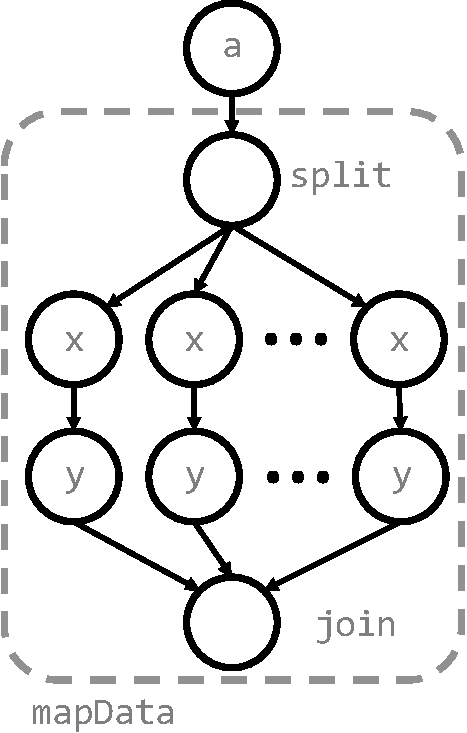
\includegraphics[width=\linewidth]{figs/graphExample.pdf}
\end{minipage}
\caption{A conservative dependency graph \emph{(Right)} resulting from one execution through a simple program \emph{(Left)}.}
\label{fig:graphExample}
\end{figure}

By construction, this graph is an overly-conservative dataflow dependency graph: if random choice $\reparamVar_a$ flows into random choice $\reparamVar_b$ (or observation $\observedVar_c$), then a path $\reparamVar_a \to \reparamVar_b$ (or $\reparamVar_a \to \observedVar_c$) exists in the graph. The converse is not necessarily true (i.e. there can exist edges between nodes that have no dataflow dependency). Note also that, by construction, the existence of a path $\reparamVar_a \to \reparamVar_b$ implies that $\reparamVar_b$ was sampled after $\reparamVar_a$ in the program execution order.

From the perpective of a random choice node $\reparamVar_i$, the graph nodes can be partitioned into the following subsets:
%%%
\begin{itemize}
\item{$\mathcal{D}_i$: the nodes ``downstream'' from $\reparamVar_i$ (i.e. the set of all nodes $d$ for which an edge $\reparamVar_i \to d$ exists.}
\item{$\mathcal{U}_i$: the nodes ``upstream'' from $\reparamVar_i$ (i.e the set of all nodes $u$ for which an edge $u \to \reparamVar_i$ exists.}
\item{$\mathcal{C}_i$: the set of nodes which are in neither $\mathcal{D}_i$ nor $\mathcal{U}_i$.}
\end{itemize}
%%%
Figure~\ref{fig:graphPartitions} illustrates these partitions on an example graph. For convenience, we also define $\mathcal{B}_i \equiv \mathcal{U}_i \cup \mathcal{C}_i$.

\begin{figure}[!ht]
\centering
%auto-ignore

%% Creator: Inkscape inkscape 0.91, www.inkscape.org
%% PDF/EPS/PS + LaTeX output extension by Johan Engelen, 2010
%% Accompanies image file 'graph.pdf' (pdf, eps, ps)
%%
%% To include the image in your LaTeX document, write
%%   \input{<filename>.pdf_tex}
%%  instead of
%%   \includegraphics{<filename>.pdf}
%% To scale the image, write
%%   \def\svgwidth{<desired width>}
%%   \input{<filename>.pdf_tex}
%%  instead of
%%   \includegraphics[width=<desired width>]{<filename>.pdf}
%%
%% Images with a different path to the parent latex file can
%% be accessed with the `import' package (which may need to be
%% installed) using
%%   \usepackage{import}
%% in the preamble, and then including the image with
%%   \import{<path to file>}{<filename>.pdf_tex}
%% Alternatively, one can specify
%%   \graphicspath{{<path to file>/}}
%% 
%% For more information, please see info/svg-inkscape on CTAN:
%%   http://tug.ctan.org/tex-archive/info/svg-inkscape
%%
\begingroup%
  \makeatletter%
  \providecommand\color[2][]{%
    \errmessage{(Inkscape) Color is used for the text in Inkscape, but the package 'color.sty' is not loaded}%
    \renewcommand\color[2][]{}%
  }%
  \providecommand\transparent[1]{%
    \errmessage{(Inkscape) Transparency is used (non-zero) for the text in Inkscape, but the package 'transparent.sty' is not loaded}%
    \renewcommand\transparent[1]{}%
  }%
  \providecommand\rotatebox[2]{#2}%
  \ifx\svgwidth\undefined%
    \setlength{\unitlength}{209.74371001bp}%
    \ifx\svgscale\undefined%
      \relax%
    \else%
      \setlength{\unitlength}{\unitlength * \real{\svgscale}}%
    \fi%
  \else%
    \setlength{\unitlength}{\svgwidth}%
  \fi%
  \global\let\svgwidth\undefined%
  \global\let\svgscale\undefined%
  \makeatother%
  \begin{picture}(1,1.62350037)%
    \put(0,0){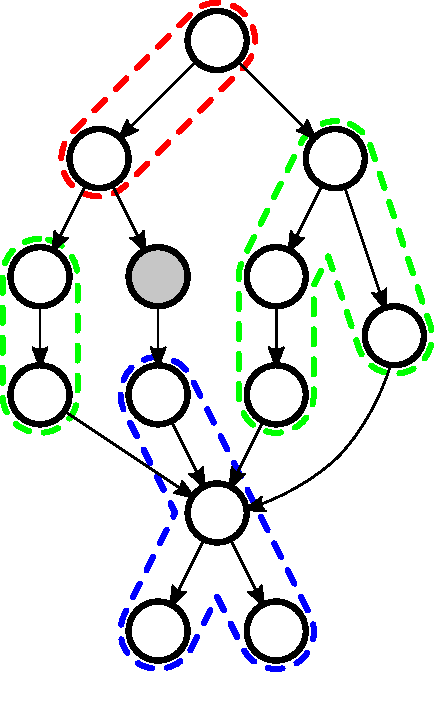
\includegraphics[width=\unitlength,page=1]{figs/graphPartitionsFig.pdf}}%
    \put(0.35075653,1.09704769){\color[rgb]{0,0,0}\makebox(0,0)[lb]{\smash{$\reparamVar_{i}$}}}%
    \put(0.42900388,0.01342784){\color[rgb]{0,0,0}\makebox(0,0)[lb]{\smash{$\mathcal{D}_{i}$}}}%
    \put(0.60518977,1.57213561){\color[rgb]{0,0,0}\makebox(0,0)[lb]{\smash{$\mathcal{U}_{i}$}}}%
    \put(0.73926511,1.38191998){\color[rgb]{0,0,0}\makebox(0,0)[lb]{\smash{$\mathcal{C}_{i}$}}}%
    \put(0.06372864,0.54981535){\color[rgb]{0,0,0}\makebox(0,0)[lb]{\smash{$\mathcal{C}_{i}$}}}%
  \end{picture}%
\endgroup%
\caption{Partitioning a dependency graph into multiple node subsets from the perspective of a random variable node $\reparamVar_i$.}
\label{fig:graphPartitions}
\end{figure}

For any given random choice $\reparamVar_i$, these partitions allows us to factor $W(\reparamVars, \observedVars)$ into three terms:
%%%
\begin{align*}
W_i(\reparamVars, \observedVars)
%
&= \log \frac{p(\xformedVars, \observedVars)}{\guide(\xformedVars | \observedVars)}\\
%
&= \log \frac{p(\mathcal{B}_i)}{\guide(\mathcal{B}_i)} + \log \frac{p( \reparamXform(\reparamVar_i) | \mathcal{B}_i)}{\guide(\reparamXform(\reparamVar_i) | \mathcal{B}_i)}	+ \log \frac{p(\mathcal{D}_i | \reparamVar_i, \mathcal{B}_i)}{\guide(\mathcal{D}_i | \reparamVar_i, \mathcal{B}_i)}\\
%
&= w_i(\mathcal{B}_i) + w_i(\reparamVar_i, \mathcal{B}_i) + w_i(\mathcal{D}_i, \reparamVar_i, \mathcal{B}_i)
\end{align*}
%%%
In the remainder of this section, we prove that the $w_i(\mathcal{B}_i)$ term can be safely removed. Specifically, we prove the following:
%%%
\begin{theorem}
For a discrete random choice $\reparamVar_i$:
\begin{equation*}
\expect_\reparamDist [ \gradparams \log \guide(\reparamXform_i(\reparamVar_i) | \reparamXform(\reparamVars_{<i}), \observedVars) w_i(\mathcal{B}_i) ] = 0
\end{equation*}
\label{thm:wterms}
\end{theorem}
%%%
In proving this theorem, the following two lemmas will be useful:
%%%
\begin{lemma}
\begin{equation*}
\reparamVars_{<i} \cap \mathcal{D}_i = \varnothing
\end{equation*}
\label{lem:depsDisjoint}
\end{lemma}
%
\begin{proof}
By definition, $\reparamVars_{<i}$ are all random choices which occur before $\reparamVar_i$ in program execution order. Also by definition, for all $d \in \mathcal{D}_i$, there exists a path $\reparamVar_i \to d$. As noted above, by construction, this implies that $d$ was created after $\reparamVar_i$ in program execution order. Thus $d$ cannot be in $\reparamVars_{<i}$.
\end{proof}
%%%
\begin{lemma}
\begin{equation*}
\guide(\reparamXform_i(\reparamVar_i) | \mathcal{B}_i) \equiv \guide(\reparamXform_i(\reparamVar_i) | \mathcal{U}_i \cup \mathcal{C}_i) = \guide(\reparamXform_i(\reparamVar_i) | \mathcal{U}_i)
\end{equation*}
\label{lem:bIndependentFromU}
\end{lemma}
%
\begin{proof}
\remark{Noah proves this. Is this pretty much just d-separation?}
\end{proof}
%
A corollary of this lemma is that $\guide(\reparamXform_i(\reparamVar_i) | \reparamXform(\reparamVars_{<i}), \observedVars) = \guide(\reparamXform_i(\reparamVar_i) | \mathcal{U}_i)$, since $\reparamVars_{<i}$ must be a subset of $\mathcal{B}_i$.
%%%
We can now prove Theorem~\ref{thm:wterms}:
%%%
\begin{align}
\expect_\reparamDist [ \gradparams \log \guide(\reparamXform_i(\reparamVar_i) | \reparamXform(\reparamVars_{<i}), \observedVars) w_i(\mathcal{B}_i) ]
%
&= \int_\reparamVars \reparamDist(\reparamVars | \observedVars) \gradparams \log \guide(\reparamXform_i(\reparamVar_i) | \reparamXform(\reparamVars_{<i}), \observedVars) w_i(\mathcal{B}_i)\nonumber\\
%
&= \int_{\mathcal{B}_i} \reparamDist(\mathcal{B}_i) w_i(\mathcal{B}_i) \sum_{\reparamVar_i} \reparamDist(\reparamVar_i | \mathcal{B}_i) \int_{\mathcal{D}_i} \reparamDist(\mathcal{D}_i | \reparamVar_i, \mathcal{B}_i) \gradparams \log \guide(\reparamXform_i(\reparamVar_i) | \reparamXform(\reparamVars_{<i}), \observedVars)\nonumber\\
%
\label{eq:wterms_depsDisjoint}
&= \int_{\mathcal{B}_i} \reparamDist(\mathcal{B}_i) w_i(\mathcal{B}_i) \sum_{\reparamVar_i} \reparamDist(\reparamVar_i | \mathcal{B}_i) \gradparams \log \guide(\reparamXform_i(\reparamVar_i) | \reparamXform(\reparamVars_{<i}), \observedVars) \int_{\mathcal{D}_i} \reparamDist(\mathcal{D}_i | \reparamVar_i, \mathcal{B}_i)\\
%
\label{eq:wterms_isDiscrete}
&= \int_{\mathcal{B}_i} \reparamDist(\mathcal{B}_i) w_i(\mathcal{B}_i) \sum_{\reparamVar_i} \guide(\reparamXform_i(\reparamVar_i) | \mathcal{B}_i) \gradparams\log \guide(\reparamXform_i(\reparamVar_i) | \reparamXform(\reparamVars_{<i}), \observedVars) \cdot 1\\
%
\label{eq:wterms_bIndependentFromU}
&= \int_{\mathcal{B}_i} \reparamDist(\mathcal{B}_i) w_i(\mathcal{B}_i) \sum_{\reparamVar_i} \guide(\reparamXform_i(\reparamVar_i) | \mathcal{U}_i) \gradparams \log \guide(\reparamXform_i(\reparamVar_i) | \mathcal{U}_i)\\
%
&= \int_{\mathcal{B}_i} \reparamDist(\mathcal{B}_i) w_i(\mathcal{B}_i) \expect_{\guide} [ \gradparams \log \guide(\reparamXform_i(\reparamVar_i) | \mathcal{U}_i) ]\nonumber\\
%
\label{eq:wterms_zeroexp}
&= \int_{\mathcal{B}_i} \reparamDist(\mathcal{B}_i) w_i(\mathcal{B}_i) \cdot 0 = 0
\end{align}
%%%
Line~\ref{eq:wterms_depsDisjoint} uses Lemma~\ref{lem:depsDisjoint}.
Line~\ref{eq:wterms_isDiscrete} uses the fact that $\reparamVar_i$ is discrete.
Line~\ref{eq:wterms_bIndependentFromU} uses Lemma~\ref{lem:bIndependentFromU} and its corollary.
Finally, line~\ref{eq:wterms_zeroexp} uses Lemma~\ref{lem:zeroexp}. 

We should note that similar methods to our removal of terms from $W$ have been used by prior work to reduce variance in LR gradient estimators. Rao-blackwellization, using the Markov blanket of a node in a graphical model, produces a similar estimator~\cite{BBVI}. In deep generative models, a similar technique allows the derivation of lower-variance estimators for each layer of the deep generative network~\cite{NVIL}. Finally, less conservative (i.e. exact) dependency graphs can be used to reduce gradient variance in stochastic computation graphs~\cite{StochasticComputationGraphs}.

\subsection{Variance Reduction Step 2: Baselines}

Next, we prove that subtracting a constant baseline term $b_i$ from every $w_i$ does not change the expectation in Equation~\ref{eq:finalEstimator}:
%%%
\begin{align*}
\expect_\reparamDist [ \gradparams \log \guide(\reparamXform_i(\reparamVar_i) | \reparamXform(\reparamVars_{<i})) (w_i(\reparamVars, \observedVars) - b_i) ]
%
&= \expect_\reparamDist [ \gradparams \log \guide(\reparamXform_i(\reparamVar_i) | \reparamXform(\reparamVars_{<i})) w_i(\reparamVars, \observedVars) ] - \expect_\reparamDist[ \gradparams \log \guide(\reparamXform_i(\reparamVar_i) | \reparamXform(\reparamVars_{<i})) b_i ]\\
%
&= \expect_\reparamDist [ \gradparams \log \guide(\reparamXform_i(\reparamVar_i) | \reparamXform(\reparamVars_{<i})) w_i(\reparamVars, \observedVars) ] 
\end{align*}
%%%
Where the last step makes use of Lemma~\ref{lem:zeroexp2}.

In our system, we use $b_i = \expect[ w_i ]$, which we estimate with of a moving average of the samples used to compute gradients. While this choice of $b_i$ is not guaranteed to reduce variance, it often does in practice, and previous systems for variational inference and reinforcement learning have exploited it~\cite{BBVI,StochasticComputationGraphs,VarianceReduction}. Another option is to \emph{learn} $b_i$, for example as a neural net function of $\observedVars$~\cite{NVIL}. The proof above also permits $b_i$ to be a function of $\reparamVars_{<i}$ (i.e. all previous random choices), which could reduce variance further by tracking posterior dependencies. This is a promising avenue for future work.

\subsection{Variance Reduction Step 3: Zero Expectation $q$ Factors}

Finally, we prove that we can remove any factors corresponding to discrete (i.e. non-reparameterized choices) from the $\gradparams \log \guide(\xformedVars | \observedVars)$ term in Equation~\ref{eq:hybridEstimator} without changing its expectation:
%%%
\begin{equation*}
\expect_\reparamDist [ \gradparams \log \guide(\reparamXform_i(\reparamVar_i) | \reparamXform_{<i}(\reparamVars_{<i}), \observedVars) ]
%
= \expect_\reparamDist [ \gradparams \log \reparamDist(\reparamVar_i | \reparamVars_{<i}, \observedVars) ]
%
= 0
\end{equation*}
where we have used Lemma~\ref{lem:zeroexp2} and the fact that $\reparamDist = \guide$ and $\reparamXform$ is the identity for discrete random choices.
%%%
